\renewcommand{\theequation}{\theenumi}
\begin{enumerate}[label=\arabic*.,ref=\thesubsection.\theenumi]
\numberwithin{equation}{enumi}
%
\item Do the points $\vec{A}=\myvec{3\\2}, \vec{B}=\myvec{-2\\-3}, \vec{C}=\myvec{2\\3} $ form a triangle?  If so, name the type of triangle formed.
%
\\
\solution The direction vectors of $AB$ and $BC$ are 
\begin{align}
\vec{A}-\vec{B} &= \myvec{5\\5}
\\
\vec{B}-\vec{C} &= \myvec{4\\6}
\end{align}
%
Since 
%
\begin{align}
\vec{A}-\vec{B} \ne k\brak{\vec{B}-\vec{C}},
\end{align}
%
the points are not collinear and form a triangle.  An alternative method is to create the matrix
\begin{align}
\myvec{\vec{A}^T\\\vec{B}^T &= \myvec{5\\5}
\\
\vec{B}-\vec{C} &= \myvec{4\\6}
\end{align}

The following code plots Fig. \ref{fig:check_tri}
%
\begin{lstlisting}
codes/triangle/check_tri.py
\end{lstlisting}
%
\begin{figure}[!ht]
\includegraphics[width=\columnwidth]{./triangle/figs/check_tri.eps}
\caption{}
\label{fig:check_tri}
\end{figure}
%
\item Find the area of a triangle whose vertices are \myvec{1\\-1}, \myvec{-4\\6} and \myvec{-3\\-5}.
%
\item Find the area of a triangle formed by the vertices $\vec{A}=\myvec{5\\2}, \vec{B}=\myvec{4\\7}, \vec{C}=\myvec{7\\-4}$.
\item Find the area of a triangle formed by the points $\vec{P}=\myvec{-1.5\\3}, \vec{Q}=\myvec{6\\-2}, \vec{R}=\myvec{-3\\4}$.
\item Are the points 
\begin{align}
\vec{A} = \myvec{3\\6 \\9},
\vec{B} = \myvec{10\\20 \\30},
\vec{C} = \myvec{25\\ -41\\5},
\end{align}
%
the vertices of a right angled triangle?
%
\item In $\triangle ABC$, Show that the centroid 
\begin{align}
\vec{O} = \frac{\vec{A}+\vec{B}+\vec{C}}{3}
\end{align}
%
\item The centroid of a $\triangle ABC$ is at the point \myvec{1\\1\\1}.  If the coordinates of $\vec{A}$ and $\vec{B}$ are \myvec{3\\-5\\7} and \myvec{-1\\7\\-6}, respectively, find the coordinates of the point $\vec{C}$.
%
\item Show that the points 
\begin{align}
\vec{A} = \myvec{2\\-1 \\1},
\vec{B} = \myvec{1\\-3 \\-5},
\vec{C} = \myvec{3\\ -4\\-4}
\end{align}
%
are the vertices of a right angled triangle.
%
\item (Cauchy-Schwarz Inequality:) Show that 
%
\begin{align}
\abs{\vec{a}^T\vec{b}} \le \norm{\vec{a}}\norm{\vec{b}}
\end{align}
%
%
\item (Triangle Inequality:) Show that 
%
\begin{align}
\norm{\vec{a}+\vec{b}} \le \norm{\vec{a}}+\norm{\vec{b}}
\end{align}
%
\item Find the area of a triangle having the points
%
\begin{align}
\vec{A} = \myvec{1\\1 \\1},
\vec{B} = \myvec{1\\2 \\3},
\vec{C} = \myvec{2\\ 3\\1}
\end{align}
%
as its vertices.

\end{enumerate}
%
